\section{Integrating Mathematical Software Systems via the Math-in-the-Middle Approach}

% Mathematics has a rich notion of data: it can be either numeric or symbolic data;
% knowledge about mathematical objects given as statements (definitions, theorems or
% proofs); or software that computes with these mathematical objects. All this data is
% really a common resource, and should be maintained as such


To achieve the goal of assembling the ecosystem of mathematical software systems in the
\pn project into a coherent mathematical VRE, we have to make the systems interoperable at
a mathematical level. In particular, we have to establish a common meaning space that
allows to share computation, visualization of the mathematical concepts, objects, and
models (COMs) between the respective systems. Building on this we can build a VRE with
classical IDE techniques. 

Concretely, the problem is that the software systems in \pn have their own representations
of and functionalities for the COMs involved. This starts with simple naming issues (e.g.\
elliptic curves are named \lstinline|ec| in the \LMFDB, and as \lstinline|EllipticCurve|
4bin \Sage), persists through the underlying data structures (five-tuple of natural numbers
for the Weierstrass equation in the \LMFDB and \ednote{MK: how in \Sage? Find a system
  where this is really different}), and becomes virulent at the level of algorithms, their
parameters, and domains of applicability.

To obtain a common meaning space for a VRE, we have the three well-known approaches in
Figure~\ref{fig:interop}
\begin{figure}[ht]\centering
  \begin{tabular}{|c|c|c|}\hline
    peer to peer & open standard & industry standard\\\hline
    \documentclass{standalone}
\usepackage{tikz}
\begin{document}
    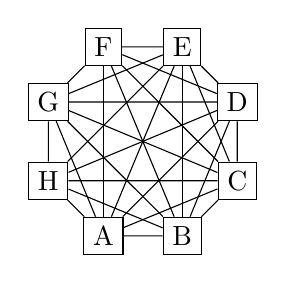
\begin{tikzpicture}
      \node[draw] (a) at (0,.3) {A};
      \node[draw] (b) at (1,.3) {B};
      \node[draw] (c) at (1.7,1) {C};
      \node[draw] (d) at (1.7,2) {D};
      \node[draw] (e) at (1,2.7) {E};
      \node[draw] (f) at (0,2.7) {F};
      \node[draw] (g) at (-.7,2) {G};
      \node[draw] (h) at (-.7,1) {H};
      \draw (a) -- (b) -- (c) -- (d) -- (e) -- (f) -- (g) -- (h) -- (a);
      \draw (a) -- (c) -- (h) -- (d) -- (g) -- (e);
      \draw (b) -- (h);
      \draw (b) -- (f);
      \draw (b) -- (d);
      \draw (b) -- (g);
      \draw (b) -- (e);
      \draw (h) -- (e);
      \draw (d) -- (f);
      \draw (g) -- (c);
      \draw (a) -- (d);
      \draw (a) -- (e);
      \draw (a) -- (f);
      \draw (a) -- (g);
      \draw (e) -- (c);
      \draw (c) -- (f);
    \end{tikzpicture}
\end{document}
%%% Local Variables: 
%%% mode: latex
%%% TeX-master: t
%%% End: 
 & \documentclass{standalone}
\usepackage{tikz}
\begin{document}
    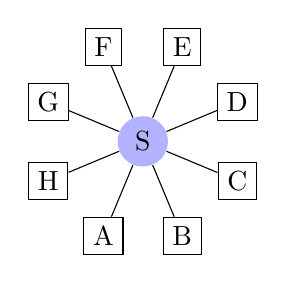
\begin{tikzpicture}
      \node[draw] (a) at (0,.3) {A};
      \node[draw] (b) at (1,.3) {B};
      \node[draw] (c) at (1.7,1) {C};
      \node[draw] (d) at (1.7,2) {D};
      \node[draw] (e) at (1,2.7) {E};
      \node[draw] (f) at (0,2.7) {F};
      \node[draw] (g) at (-.7,2) {G};
      \node[draw] (h) at (-.7,1) {H};
      \node[circle,fill=blue!30] (m) at (.5,1.5) {S};
      \draw (m) -- (a);
      \draw (m) -- (b);
      \draw (m) -- (c);
      \draw (m) -- (d);
      \draw (m) -- (e);
      \draw (m) -- (f);
      \draw (m) -- (g);
      \draw (m) -- (h);
    \end{tikzpicture}
\end{document}
%%% Local Variables: 
%%% mode: latex
%%% TeX-master: t
%%% End: 
 & \documentclass{standalone}
\usepackage{tikz}
\begin{document}
    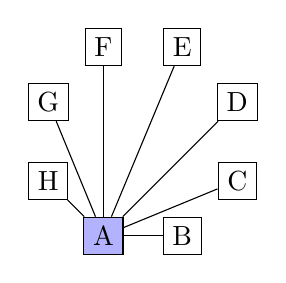
\begin{tikzpicture}
      \node[draw,fill=blue!30] (a) at (0,.3) {A};
      \node[draw] (b) at (1,.3) {B};
      \node[draw] (c) at (1.7,1) {C};
      \node[draw] (d) at (1.7,2) {D};
      \node[draw] (e) at (1,2.7) {E};
      \node[draw] (f) at (0,2.7) {F};
      \node[draw] (g) at (-.7,2) {G};
      \node[draw] (h) at (-.7,1) {H};
      \draw (a) -- (b);
      \draw (a) -- (c);
      \draw (a) -- (d);
      \draw (a) -- (e);
      \draw (a) -- (f);
      \draw (a) -- (g);
      \draw (a) -- (h);
    \end{tikzpicture}
\end{document}
%%% Local Variables: 
%%% mode: latex
%%% TeX-master: t
%%% End: 
\\\hline
    $n^2/2$  translations & $2n$ translations & $2n-2$ translations \\
    symmetric & symmetric & asymmetric\\\hline
  \end{tabular}
  \caption{Approaches for Safe Distributed Computation/Storage/UIs}\label{fig:interop}
\end{figure}
The first does not scale to a project with about a dozen systems, for the third there is
no obvious contender in the \ODK ecosystem. Fortunatly, we already have a ``standard'' for
expressing the meaning of COMs -- \defemph{mathematical vernacular}: the language of
mathematical communication, and in fact all the COMs supported the \ODK VRE are documented
in mathematical vernacular in journal articles, manuals, etc.

The obvious problem is that mathematical vernacular is too 
\begin{inparaenum}[\em i\rm)]
\item \emph{ambiguous}: we need a human to understand structure, words, and symbols
\item \emph{redundant}: every paper introduces slightly different notions. 
\end{inparaenum}
Therefore we adopt an approach, where we partially formalize (\defemph{flexiformalize})
mathematical vernacular to obtain a flexiformal ontology of mathematics that can serve as
an open communication vocabulary. We call the approach the \defemph{Math-in-the-Middle}
(MitM) Strategy for integration and the ontology the MitM ontology\ednote{MK: I do not
  like this yet!}. In the \ODK project we want to use the OMDoc/MMT\ednote{MK: cite}
format for this (see ???\ednote{where?})

\begin{wrapfigure}r{4cm}\vspace*{-1.5em}
  \documentclass{standalone}
\usepackage[mh]{mikoslides}
% this file defines root path local repository
\defpath{MathHub}{/Users/kohlhase/localmh/MathHub}
\mhcurrentrepos{MiKoMH/talks}
\libinput{WApersons}
% we also set the base URI for the LaTeXML transformation
\baseURI[\MathHub{}]{https://mathhub.info/MiKoMH/talks}

\libinput{preamble}
\begin{document}
    \begin{tikzpicture}[scale=1.3]
      \tikzstyle{withshadow}=[draw,drop shadow={opacity=.5},fill=white]
      \tikzstyle{system}=[draw]
      \tikzstyle{standard}=[circle,fill=blue!30]
      \tikzstyle{interface}=[circle,fill=purple!30,inner sep = 1pt,]
      \node[system] (a) at (0,.3) {A};
      \node[system] (b) at (1,.3) {B};
      \node[system] (c) at (1.7,1) {C};
      \node[system] (d) at (1.7,2) {D};
      \node[system] (e) at (1,2.7) {E};
      \node[system] (f) at (0,2.7) {F};
      \node[system] (g) at (-.7,2) {G};
      \node[system] (h) at (-.7,1) {H};
      \node[standard] (m) at (.5,1.5) {S};
      \node[interface] (ia) at (0.2,.9) {a};
      \node[interface] (ib) at (.8,.9) {b};
      \node[interface] (ic) at (1.1,1.2) {c};
      \node[interface] (id) at (1.1,1.75) {d};
      \node[interface] (ie) at (.8,2.1) {e};
      \node[interface] (if) at (0.2,2.1) {f};
      \node[interface] (ig) at (-.1,1.75) {g};
      \node[interface] (ih) at (-.1,1.2) {h};
      \draw (m) -- (ia) -- (a);
      \draw (m) -- (ib) -- (b);
      \draw (m) -- (ic) -- (c);
      \draw (m) -- (id) -- (d);
      \draw (m) -- (ie) -- (e);
      \draw (m) -- (if) -- (f);
      \draw (m) -- (ig) -- (g);
      \draw (m) -- (ih) -- (h);
      \begin{pgfonlayer}{background}
        \node[draw,cloud,fit=(ia) (ib) (ic) (id) (ie) (if) (ig) (ih),
                   inner sep=-7pt,withshadow] (st) {};
        \node[fit=(d) (id),ellipse,inner sep=-1pt,rotate=20,draw,dashed,red] (sys) {};
      \end{pgfonlayer}
      \end{tikzpicture}
\end{document}
%%% Local Variables: 
%%% mode: latex
%%% TeX-master: t
%%% End: 
\vspace*{-.5em}
  \caption{Interface theories}\label{fig:interface-theories}\vspace*{-1em}
\end{wrapfigure}
Before we go into any detail about how this ontology looks and how it induces a uniform
meaning space, we have to address another problem: the descriptions in the MitM ontology
must at the same time be system-near, to make interfacing easy for systems, and serve as
an interperability standard -- i.e. be general and stable. If we have an ontology system
that allows modular/structured ontologies, we can solve this apparent dilemma by
introducing \defemph{interface theories}, i.e. ontology modules (the light purple circles
in Figure~\ref{fig:interface-theories}) that are at the same time system-specific in their
description of COMs -- near the actual representation of the system and part of the
greater MitM ontology (depicted by the cloud in Figure~\ref{fig:interface-theories}) as
they are connected to the core MitM ontology (the blue circel) by views we call
\defemph{interviews}\ednote{MK: I am not sure I like this word either}. The MitM approach
stipulates that interface theories and interviews maintained and released together with
the respective systems, whereas the core MitM ontology represents the mathematical scope
of the VRE and is maintained with it. In fact in many ways, the core MitM ontology is the
conceptual essence of the mathematical VRE. 




\ednote{MK: continue, essentially the St.\
  Andrews stuff}

%%% Local Variables:
%%% mode: latex
%%% TeX-master: "paper"
%%% End:

%  LocalWords:  pn visualization lstinline ec lstinline Weierstrass ednote
